\documentclass{article}
\title{Generating Efficient Interpreters}
\author{
    Marcel Taubert  (mt652)\\
    20962335        \\
    \\
    School of Computing \\
    MSc Advanced Computer Science\\
    University of Kent \\
    \\
    Supervisor: Dr. Michael Vollmer
}
\usepackage{natbib,hyperref}
\usepackage{graphicx}
\date{\today}
\begin{document}
\maketitle
\clearpage
\tableofcontents
\section{Introduction}

%1. Introduction: objectives, intro to contents (overview)
    %- what is a vm interpreter
    %- how does a vm interpreter work
    %- difference between stack and register based vm
    %- what are optimizations, what optimizations are we using
    %- what kind of optimizations are there
    %- code generation (from a config file)
%3. description of the problem
    %- many parts of interpreter writing can be automated 
    %- why should we care about efficieny in interpreter
%6. literature and technology review, (what papers, vmgen??)
    %- what it says and how it relates to my project
%7. possible approaches and reason why we choose this approach
    %- by hand is hard
    %- doing it automatically
    %- what optimizations
    %- why rust not C (why others did it in C, what can you do in C)
    %- why for the Imp programming language
    %- why not compile to C code (2nd paper)
%8. description of work that we did 
    %- vm (stack, why tho)
    %- interpreter (visitor pattern)
    %- parser and scanner (not generated, why)
    %- bytecode design (why and how does it work)
    %- bytecode generator
    %- bytecode interpreter (visitor pattern)
    %- what is the input language
    %- optimizations (superinstructions, computed go-to)
    %- benchmark program
%10. Results: tests, benchmarks, what kind of programs
%11. Summary, Conclusion
%12. future work (automation)
%13. Bibliography

%/*
%What is an interpreter?
%- Programming is everywhere
%- 2 ways how code is run (compiler and interpreter)
%- whats good about interpreters
%*/

In today's modern world, everything operates through code. We all use
technology that's powered by code, whether we realize it or not. However, most
individuals, including a substantial number of programmers, lack an
understanding of how the code is executed on their devices.

\subsection{What is an interpreter?}

In general, there are two approaches to executing code. Both methods involve
translating the human-readable code into a more abstract form that the computer
can understand.

The first technique describes the process of code being compiled (translated)
into machine code. The end product is a stand-alone program that can be
executed at any time on the architecture it was compiled for.

The second approach is called 'interpreting'. There are two primary methods for
how an interpreter works. One approach is called a tree-walk interpreter. In
this case, the interpreter just walks the generated abstract syntax tree and
executes it. The second approach is a virtual machine interpreter which
involves an extra step between the generation of the syntax tree and the
execution. A compiler walks the tree and generates byte code. This bytecode
will then be fed into the virtual machine which executes it. We will use a
virtual machine interpreter in this paper. Interpreters are generally easier to
implement and have some other advantages that make them more approachable than
compilers like portability or a fast edit-compile-run cycle as stated by the
authors of vmgen ~\cite{vmgen}. 

%/*
%what is a vm interpreter?
%- create intermediate representation that is similar to a real machine
%- series of bytecode instructions
%- (Frontend) compiler that produces this bytecode (written in rust)
%- (Backend) vm interpreter that executes the instructions
%- Some examples of vm interpreters (JVM, PVM (python))
%*/

\subsection{What is a virtual machine interpreter?}
A famous technique to implement interpreters is to build a virtual machine
interpreter. A VM interpreter is generally divided into two systems. A frontend
and a backend. ~\cite{vmgen}

The frontend consists of a compiler that takes the written code and produces a
sequence of bytecode instructions. The backend is a virtual machine that gets
the stream of bytecode instructions as input and executes them. ~\cite{vmgen}

The bytecode or intermediate representation used in a VM interpreter is usually
designed to be very similar to a real machine. ~\cite{vmgen}

Some real-world examples of virtual machine interpreters are for example the
JVM (Java Virtual Machine) or the PVM (Python Virtual Machine).


\subsection{Virtual machine}
When we are talking about virtual machines we distinguish between stack-based VMs and 
register-based VMs.

Each of the versions has its advantages and disadvantages.

Stack-based virtual machines are generally easier to implement than the register-based approach.
That shows for example the complexity of the intermediate representation used in the virtual 
machine. The stack-based bytecode tends towards being smaller and by that more efficient in 
comparison to the rather complex bytecode instructions of the register-based approach.

\begin{verbatim}
typical stack based instruction:
Push 1    -- push value to the stack
\end{verbatim}

\begin{verbatim}
typical register based instruction:
LD R1, 42 -- load value `42` into register R1
\end{verbatim}

This simplicity is the reason we have decided to rely on a stack-based virtual machine in
this paper.

\subsection{Optimizations}
Optimiztions are essential for delivering efficient and performant execution of
programs. These optimizations can be implemented by the compiler directly or
other parts of a VM interpreter such as the JIT (Just in Time) compiler, that
are more complex and we will not be covered in this paper.

Optimizations generally involve a trade-off in compilation time and memory
against execution speed. This results of additional passes on the generated
byte code for example that are needed to implement certain optimizations.

During the development of this project we have looked at a number of different
optimizations. Some of the optimizations that we have implemented for the
project are threaded code inside of the interpreter and superinstructions in
the compiler.

\subsection{Automation}
Writing an interpreter for a programming language can be a tedious and
challenging task on its own. Thinking about how to keep the code efficient and
implement optimizations makes it even harder.

One solution to this is automating the process of writing a virtual machine
interpreter.

This would prevent many error sources such as human errors and lead to enhanced
code quality. By eliminating the manual writing work, the programmer can focus
on higher-level aspects of the project.

Due to quicker development cycles, the interpreter can be fine-tuned without
needing to change the code and be more efficient.

\subsection{Objectives}
This paper will use the Rust programming language to build each part of a virtual machine 
interpreter with the eventual goal of automating the generation of it self depending on
a given configuration.

We will explore techniques and approaches on how to build a VM interpreter in
Rust and use benchmarking to visualize results highlighting effects of
optimizations.

\section{Description of the problem}
When it comes to the problem that we are trying to solve there are two main
points: efficiency and automation.

\subsection{Efficiency}
In terms of efficiency at run time, nativ compiled machine code will always
outperform the interpreted version. So why would we even care about writing
efficient interpreters and not just use native code compilers.

One of the main reasons interpreters are preferred over compilers is that 
native code compilers are more complex to develop and difficult to maintain.
~\cite{structure_and_performance}

Another big advantage of the interpreting approach is that compilers can only
generate native code for one target system while the virtual machine
interpreter stays consistent on every system. By that the interpreter is
portable and the generated code does not depend on the underlaying machine.

Summed up, the first problem is that interpreters will never be as fast as
native compiled machine code but by contributing to the increase of efficiency
we get all the benefits of using interpreters while minimizing the
disadvantages to compilers.

\subsection{Automation}
Many programmers will have the idea of implementing their own programming
language at some point in their career. Most of them will have noticed that
buidling an interpreter is a challenging task and requires a lot of work and
a clear structure. In addition to that it shows that many parts of an VM
interpreter are similar and repetitive. For example the code for executing 
VM instructions will be similar for most of the instructions. ~\cite{vmgen}

But what happens when the interpreter does not give the expected outcome in
terms of efficiency. It results in manual rewriting of a codebase just to
change the implementation of some part of the VM interpreter to see if the
performance increases. Rewriting the whole interpreter to test if the
performance is better using a different development approach is not only time
consuming but also error prone.

One solution to this problem is automation. The developer should be able to
provide a configuration file and based on that we will generate an efficient VM
interpreter. It will already use efficient implementation techniques and come
with built in optimizations. It also provides easy extensibility for the user
without needing to change any source code.

\section{Literature review}
This literature review compiles a selection of influential papers that explore
various aspects of efficient interpreter design or the generation of them. 

By analyzing these papers, we aim to highlight different appraoches and
concepts used to develop efficient interpreters and analyze them regarding
complexity.

We'll cover the choice of programming language, multiple ways the interpreter
can be implemented, types of virtual machines and the output format of the
compiler.

\subsection{Programming Language}
Most of the code written, targeting the problem of efficent interpreters or
compilers is either written in C or directly in assembly language.

But why are developers using languages such as C when it is known to be error
prone or even assembly which is known to be even more complex and hard to
maintain.

The reason for this is abstraction. Languages such as Python or Java are so
easy to write because the langauge itself provides many layers of abstraction
from what is actually hapening on the machine level. This makes it easier for
the programmer to write safe code. 

The downside of this abstraction is that it limits the contol the programmer
has over the system.

In compiler development there are many situations where it is crucial for the
programmer to be able to use little tricks on the lowest layers of the system
to reach a maximum performance gain.

In the paper "Optimizing an ANSI C Interpreter with Superoperators" the author
Todd A. illustrates the superiority of assembly by writing:

\begin{quotation}
"The interpreter is implemented in assembly language.
Assembly language enables important optimizations like keeping the evaluation
stack pointer and interpreter program counter in hardware registers." ~\cite{superoperators}
\end{quotation}

Another example of an optimization that is complicated to implement in high
level languages such as Python but easy to implement in assembly and in some
versions of C is the threaded code or computed goto optimization.

As a limitation to C the authors of 'vmgen - A Generator of Efficient Virtual
Machine Interpreters' state:
\begin{quotation} 
"This technique cannot be implemented in ANSI C, but it can be implemented in
GNU C using the labels-as-values extension." ~\cite{vmgen} 
\end{quotation}

\subsection{Interpreter approaches}
There are several ways to implement an interpreter. We are looking
at the 2 most widely used practices. 
Both of them start in the parsing phase by creating an Abstract Syntax
Tree (AST). The tree consists of nodes each representing a construct in
the programming language, for example a statement or an expression.

The tree walk interpreter is the simplest way to create an interpreter when the
AST is already built. As the name suggests it traverses the tree and when it
encounters a node it executes the corresponding operation.

Tree walk interpreters are easy from the viewing point of the implementor. The
tree closely mirrors the structure of the source code and by that makes errors
easier to debug in the tree structure.

This simplicity comes with the cost of reduced performance. One reason why a
tree walk interpreter is slower than a bytecode interpreter is that as they
traverse the tree they perform execution for each node wich can result in
redundant operations. Furthermore it is hard to use optimizations, since
it directly executes the nodes.

Bytecode interpreters are traversing the AST and building up a sequence of 
instructions which then will be executed. 

The step of creating an intermediate reprentation (IR) opens up a new way to
operate on the code. Now that we work with a series of instructions instead of
a tree of nodes we can perform all sorts of optimizations on it.

This makes the bytecode interpreter more efficient. It also makes it more
complex since now we have to generate bytecode, implement optimizations
and execute the bytecode instructions. Debugging is also more complex since
the generated instructions do not mirror the code structure anymore.

\subsection{Virtual Machines}
Virtual machines create an abstraction layer between the host machine and 
the code that is executed. This enables machine independence for code
written in programming languages that do not run on a certain architecture.

The paper 'An introduction to the UCSD PASCAL system' describes the development
of an early virtual machine, pseudomachine, to enable the use of high level
programming languages such as FORTRAN on unsupported systems. During that time
it was common for new architectures to support popular languages like FORTRAN
but even then, there were many problems when transporting programs from one
system to another and smaller machines had no support of high level languages.
~\cite{pascal}

When talking about virual machines we only consider the 2 main paradigms in
this paper, namely stack based and register based virtual machines.

While virtual machines are great to use in combination with interpreters
each architecture has it's advantages and disandvantages.

Stack based virtual machines use a stack to manage state. The stack pointer,
often abbreviated with sp, is used to keep track of the top of the stack.
Instructions like PUSH and POP can manipulate the stack by adding or removing
values from it while incrementing or decrementing the stack pointer.

The main advantage of a stack-based virtual machine lays in it simplicity.
The implementation is straight forward, the instructions are kept simple
and optimiztions are easy to implement.

Register based virtual machines work on a different principle. They use a set of
virtual registers which are designed to mimic hardware registers as a place to
store data. Instructions such as LOAD or STORE can modify the registers.

The instructions used in register based virtual machines are larger since they
need to encode the operands. As an example the STORE instrucion needs to know 
the value to store and the register where it should store the value.

The execution cycle involve 3 steps. Fetching, decoding and executing. First
the machine needs to get the instruction from memory. Then it needs to decode
the instruction to know which operation to perform and which registers to use.
This decoding step can add a small overhead to the machine but since it usually
involves just simple logical operations it is still very fast. In the last step
the operation is executed and the registers are modified accordingly.

Since all operations are performed on registers, the need to push and pop from
the stack is eliminated which results in efficient data access.

Regarding the effort it takes to create an efficient register based virtual
machine interpreter M. Anton Ertl says:

\begin{quotation}
"From the view of the compiler writer, many languages can be easily compiled for
stack machine code. To achieve better performance with a register machine, the
compiler must perform optimizations, e.g., global register allocation (which
needs data flow analysis). This would eliminate one of the advantages of using an
interpreter, namely simplicity." ~\cite{stack_caching_for_interpreters}
\end{quotation}

A good example to compare stack based virtual machines with register based
machines on a real world project is Lua. Lua runs it's programs on a virtual
machine interpreter and therefore compiles the code into instructions for a
virtual machine.

When Lua was first created in 1993 it used a stack based virtual machine. 10
years later in 2003 with the release of Lua 5.0 they have changed their
approach and now use a register based VM. ~\cite{lua_implementation}

To understand how Lua profited from the register based virtual machine we first
need to understand how Lua works.

Lua creates a prototype for each function in the code. The prototype contains an
array with all the instructions to execute this function and an array of all the
Lua values and constants used. ~\cite{lua_implementation}

Upon entering a function, an activation record is preallocated on the stack.
This record holds all funcion registers, where local variables are stored.
Resulting in efficient variable access. ~\cite{lua_implementation}

In addition to that register based instructions do not need any PUSH or POP
instruction which are expensive in Lua because of the way Lua represents
values.

Looking at the disadvantages of register based VMs tn terms of generated code
size and single instruction size in Lua we can see that they are not too bad.

Lua's stack based virtual machine had an instruction set of 49 instructions
where the register based approach only needed 35. The size of a single
instruction increased from 2 bytes to 4 bytes with the change of the virutal
machine architecture but this relativises itself due to less generated
instructions.

Here an example:

\begin{figure}[ht]
    \begin{verbatim}
        local a,t,i
        a = a+i
        a = a+1
        a = t[i]
    \end{verbatim}
    \caption{\textit{Example Lua code from ~\cite{lua_implementation}}}
    \label{fig:lua_code}
\end{figure}

The generated instructions vary a lot from Lua 4.0 to Lua 5.0.

\begin{figure}[ht]
    \begin{verbatim}
        PUSHNIL     3
        GETLOCAL    0
        GETLOCAL    2
        ADD
        SETLOCAL    0
        GETLOCAL    0
        ADDI        1
        SETLOCAL    0
        GETLOCAL    1
        GETINDEXED  2
        SETLOCAL    0
    \end{verbatim}
    \caption{\textit{Generated instructions for Lua 4.0 (stack based VM) from ~\cite{lua_implementation}}}
    \label{fig:lua_generated4}
\end{figure}


\begin{figure}[ht]
    \begin{verbatim}
        LOADNIL     0 2 0
        ADD         0 0 2
        ADD         0 0 250 ;1
        GETTABLE    0 1 2
    \end{verbatim}
    \caption{\textit{Generated instructions for Lua 5.0 (register based VM) from ~\cite{lua_implementation}}}
    \label{fig:lua_generated5}
\end{figure}

Comparing Figure \ref{fig:lua_generated4} and Figure \ref{fig:lua_generated5}
we can see even though each instruction in Figure \ref{fig:lua_generated5} has 3 operands,
resulting in larger size, it just generated a total of 4 instructions compared
to 11 in Figure \ref{fig:lua_generated4}.

\subsection{Output Format}
The frontend of the interpreter, the compiler, generates output. What kind
of output it is depends on the use case.

For example, for virtual machine interpeters the compiler outputs byte code that
can be run by the virutal machine. This is platform independent but comes with
the cost of reduced performance.

A native-code compiler outputs machine code for a specific architecture. This is faster
than interpreting but is limited when it comes to portability.

Another approach is to compile to C. With that we have portability and gain all the 
optimization that were added to C compiler in the last 30 years. Some disadvantages
are stated by the authors of 'The Structure and Performance of Efficient Interpreters':

\begin{quotation} 
"Why not write a compiler to C? While this method addresses the
ease-of-implementation and retargeting issues, it is not acceptable when
interactivity, quick turnarounds, or non-C features (e.g., run-time
code-generation or guaranteed tail-call optimization) are required."
~\cite{structure_and_performance}
\end{quotation} 

The paper 'Optimizing an ANSI C Interpreter with Superoperators' shows a hybrid
approach which generates "efficient code that includes a small amout of native
code with interpreted code". ~\cite{superoperator}

\begin{quotation}
"This hybrid approach allows the object files to maintain all C calling con-
ventions so that they may be freely mixed with natively compiled object
files. The interpreted object code is approximately the same size as
equivalent native code, and runs only 3-16 times slower." ~\cite{superoperator}
\end{quotation}

\section{Approaches}
In the following section we will go into detail about why we have used the 
techniques and tools as we did, re-evaluate on the decisions and present 
learnings.

The choice of the implementation langauge had probably the most influence on
the efficiency of the VM interpreter.

The industry standard for implementing such systems is either C or assembly.
We made the decision to use Rust early on to explore how we can use it's
higher-level language features, such as it's enums, to do low level programming
and see if we can get close to the efficency of C implementations with the
convenience that Rust gives us during development.

Rust prevents many errors from happening during development by for example
enforcing strict rules on ownership of data and provides high level language
features such as iterators, match statements and a rich standard library of 
containers such as HashMaps.

To represent byte code in Rust we used it's powerful enums. This is very
convenient since enums can have fields attached and are an actual type not like
in C where enums are just numbers.

While this approach is very convenient it is not very efficient. One byte code
instruction as we designed the enum takes up 32 bits of memory.

The largest enum variant is the jump instruction as it holds a string `label`
and an i32 `offset`. Since Rust's enums behave like a tagged union every
instruction has the size of the largest instruction.

\begin{verbatim}
A string in Rust contains:
    8 bits -> pointer to the chars
    8 bits -> len of the string
    4 bits -> the i32 value
    8 bits -> enum tag
    + padding

    adds up to 32 bits.
\end{verbatim}

A more efficient approach to represent byte code in Rust would be to just
define each instruction by a unique integer. By doing this, we would use the
same technique as using enums in C and loose the convenience of using Rust's
language features.
 
A big downside that followed the decision to use Rust was the way we have
implemented the computed goto optimization. The detailed implementation is
discussed in section \ref{it:goto}.

Since rust does not allow the usage of labels like C does, we had to use an
alternative technique where we stored the function pointers to the routines
that execute a byte code instruction, in a hash map and had to use the
discriminants as an index. This additional indirection at the end of every 
executed instruction caused an extreme performance slowdown.

The typical approach in C would be to store the adderesses of the labels to the
routines in an array and index it by using the C enum reprentation of an
instruction.

Earlier we evaluated that register-based virtual machines, when set-up
correctly, can be faster and more efficient than stack based VMs.

In our implementation we still decided to use a stack based virtual machine.
The reason for that lays in its simplicity. This project aimes to explore
how to build a virtual machine interpreter in Rust. Therefore we tried to
keep the implementation as simple as possible. The possible impelementation of
a register based virutal machine in the future is more described in the Section
\ref{sec:future}.

\section{Description of work}
The goal of this project is to build a virtual machine interpreter and 
explore the implementation of such in the Rust programming language.

\subsection{Tools used}
During the development of this project we used three programming languages. 

\begin{enumerate}
    \item \textbf{Rust}:\\
        We used Rust to build all parts of the virtual machine interpreter.
    \item \textbf{Python}:\\
        We used Python to capture and visualize benchmark results using matplotlib.
    \item \textbf{Imp}:\\
        Imp is the input language the VM interpreter operates on. \ref{sec:input_language}
\end{enumerate}

\subsection{Virtual Machine}
The virtual machine, the backend of the VM interpreter, is the part that
exectues the byte code that was generated by the compiler.

\subsubsection{Implementation}
The virtual machine we have built is very basic. It contains a representation
of the stack and a HashMap to hold the global variables.

\begin{verbatim}
pub struct ByteCodeInterpreter {
    stack: Vec<usize>,
    pc: i32,
    variables: HashMap<String, usize>,
}
\end{verbatim}
\textit{ByteCodeInterpreter struct definition} \\

The optimized version of it implementing the `computed goto` optimization (see
section \ref{it:goto}) is a bit more complicated. Here we also have the mapping
of ByteCode to the function that executes this bytecode. This optimization is 
described in more detail at \ref{it:goto}.

\begin{verbatim}
pub struct ByteCodeInterpreterThreaded {
    stack: Vec<usize>,
    pc: i32,
    variables: HashMap<String, usize>,
    ops: HashMap<Discriminant<ByteCode>, Instruction>,
    instructions: Vec<ByteCode>,
}
\end{verbatim}
\textit{ByteCodeInterpreterThreaded struct definition} \\

\subsubsection{Stack}
The virtual machine we built is stack based. This means there are no registers
and all the data is handled on the stack.

When you add two numbers there will be a PUSH instruction for both values
and an ADD instruction which will pop the last two values from the stack,
adds them together and pushes the result back on the stack.

\begin{verbatim}
The code `1 + 2` would produce the following instructions:

inst:    stack:
         []
push 1   [1]
push 2   [1, 2]
add      [3]
\end{verbatim}

\subsubsection{Byte code}
\label{sec:byte_code}

To define a byte code we have decided to use Rust's powerful enums. They are
not only able to perfectly represent each instruction with it's parameters but
also helps during development due to Rust's powerful type system.

\begin{verbatim}

#[derive(Debug, Clone, PartialEq)]
pub enum ByteCode {
    Push(usize),
    Pop,
    Add,
    Sub,
    Mul,
    Var(String),
    Eq,
    NEq,
    Lt,
    Gt,
    Lte,
    Jz {
        label: String,
        offset: i32,
    },
    ...
}

\end{verbatim}
\textit{Rust representation of the Byte Code} \\

\subsection{Interpreter}
The interpreter consists of a scanner and a parser. We have decided to
handwrite both parts instead of generating them. Even though the scanner and
the parser are not the most performance critical parts of an interpreter we
decided to handwrite them in Rust to have full control over what is happening.

\subsubsection{Scanner}
The scanner was implemented very straight forward by using a match statement
inside a while loop to iterate the source code and output a stream of tokens.

Tokens are defined as the token type and an optional literal.

\begin{verbatim}
pub struct Token {
    pub token_type: TokenType,
    pub literal: Option<Object>,
}
\end{verbatim}
\textit{Token definition}

\begin{verbatim}
pub enum Object {
    Num(f64),
    Bool(bool),
    Variable(String),
    DivByZeroError,
    ArithmeticError,
}
\end{verbatim}
\textit{Object definition}

\begin{verbatim}
pub enum TokenType {
    LeftParen,
    RightParen,

    Minus,
    Plus,
    ...
    Eof,
}
\end{verbatim}
\textit{TokenType definition}

\subsubsection{Parser}
The parser takes the stream of tokens as input and builds up an Abstract Syntax
Tree (AST). In the Rust code it is represented as a `Vec<Rc<Stmt>>`.

\begin{verbatim}
As an example the code `x := 10;` will get tokenized into 
`[Identifier,Assignment, NumberLiteral, Semicolon]` 
and the parser will output a tree structure like:

ExpressionStmt {
    expr: AssignExpr {
        name: "x",
        value: LiteralExpr {
            value: Num(10)
        }
    }
}
\end{verbatim}

\subsubsection{Interpreter (testing)}
To be able to test the scanner and parser before writing the bytecode generator
we build a small interpreter that just runs the code.

It uses the visitor pattern to traverse the abstract syntax tree generated by
the parser and executes the code immediatly.

To use the visitor pattern approach we have implemented a statement visitor and
an expression visitor.

\begin{verbatim}
pub trait StmtVisitor<T> {
    fn visit_block_stmt(&self, stmt: &BlockStmt) -> Result<T, ()>;
    fn visit_if_stmt(&self, stmt: &IfStmt) -> Result<T, ()>;
    fn visit_expression_stmt(&self, stmt: &ExpressionStmt) -> Result<T, ()>;
    fn visit_print_stmt(&self, stmt: &PrintStmt) -> Result<T, ()>;
    fn visit_while_stmt(&self, stmt: &WhileStmt) -> Result<T, ()>;
}
\end{verbatim}
\textit{Statement visitor example}

For each statement we have setup a structure holding the necessary data.

\begin{verbatim}
#[derive(Debug)]
pub struct IfStmt {
    pub condition: Rc<Expr>,
    pub then_branch: Rc<Stmt>,
    pub else_branch: Option<Rc<Stmt>>,
}
\end{verbatim}
\textit{Structure holding data for an if statement}


\subsection{Optimizations}
Optimizaions play a critical role in the field of compiler design. From the
endless list of optimizations we chose a couple ones to dive into detail
about and use in the VM interpreter.

Some common techniques are:
\begin{enumerate}
    \item \textbf{Dead Code Elimination}:\\
    \label{item:dead_code_elimination}
        Remove parts of the code that are never to be used.

        Consider the follwing C code. In this case the variable `c` is never
        used. So the statement `int c = 3;` does not need to be compiled.
        \begin{verbatim}
        int main() {
            int a = 1;
            int b = 2;
            int c = 3; // never used

            return a + b;
        }
        \end{verbatim}
    \item \textbf{Constant folding}:\\
        When calcualtions are only using constant values and by that can be
        evaluated during compile time it will directly replace it with the
        computed value.

        Consider the follwing C code. In this example `int a = 10 + 20;` only uses values known
        at compile time so the compiler can internally replace the statement with `int a = 30;`.
        \begin{verbatim}
        int main() {
            int a = 10 + 20;
            printf("%d", a);

            return 0;
        }
        \end{verbatim}
    \item \textbf{Superinstructions}:\\
        Superinstructions is a term used for the case when combining two or more instructions 
        into a single big instruction.

        Consider the following C code.

        \begin{verbatim}
        int main() {
            int i = 0;
            while (i < 10) {
                i += 1;
            }
        }
        \end{verbatim}

        If we naively 'compile' this code we would get instructions like this:

        \begin{verbatim}

        // in the loop
        load i -- get the variable at i and push it to the stack
        push 1 -- push the value '1' to the stack
        add    -- pop the first 2 values from the stack, add them, and push the result back on the stack

        \end{verbatim}

        We always need 2 instructions to push the constant value to the stack and then add the top
        2 values on the stack together.

        But we can create a superinstruction called 'push\_add' which would change the generated
        code to this.

        \begin{verbatim}

        // in the loop
        load i     -- get the variable at i and push it to the stack
        push_add 1 -- superinstruction that does the push and then the add

        \end{verbatim}

        That change might seem very insignificant but we can extend this idea
        of superinstructions to combine already built superinstructions with
        each other and by that save many instructions.


    \item \textbf{Computed goto}:\\
    \label{it:goto}
        When executing the bytecode inside of a virtual machine interpreter for
        example, you will usually find a big switch statement inspecting the
        current instruction and executing it. In our case, since we used Rust
        we have a big match statement like this.

        \begin{verbatim}

        while self.pc < instructions.len() as i32 {
            let inst = &instructions[self.pc as usize];
            match inst {
                ByteCode::Push(value) => {
                    self.stack.push(*value);
                }
                ByteCode::Pop => {
                    self.stack.pop().unwrap();
                }
                ByteCode::Add => {
                    let a = self.stack.pop().unwrap();
                    let b = self.stack.pop().unwrap();
                    self.stack.push(b + a);
                }
                ...
            }
        }
        \end{verbatim}

        This `while` loop will iterate over every single instruction in the program. That means
        for every instruction it has to go through all the possible values inside of the `match`
        statement until it find the matching result.

        The `Computed goto` optimization tries to make this process more efficient.

        To implement that, we have to create an array of function pointers where
        the index of the array corresponds to an instruction or use a HashMap
        with the byte code instruction as the key and the function as a value
        like we did in Rust.

        \begin{verbatim}

        pub type Instruction = fn(interp: &mut ByteCodeInterpreterThreaded);
        ... {
            ops: HashMap<Discriminant<ByteCode>, Instruction>
        }

        ops.insert(std::mem::discriminant(&ByteCode::Push(0)), Self::op_push);
        ops.insert(std::mem::discriminant(&ByteCode::Pop), Self::op_pop);
        ops.insert(std::mem::discriminant(&ByteCode::Add), Self::op_add);
        \end{verbatim}

        Then each of the functions (Self::op\_push, Self::op\_add, ...) will finish
        with a call to a `next()` function.

        This next() function will increment the program counter (the current
        position in the byte code) and call the function which was mapped to
        the next instruction in the HashMap.

        In our case in Rust the next function looks like the following.

        \begin{verbatim}
        fn next(&mut self) {
            // incrementing the program counter;
            self.pc += 1 

            // check for end of stream
            if self.pc >= self.instructions.len() as i32 {
                return; 
            }

            // call the next function
            self.ops[&self.instructions[self.pc as usize]](self);
        }
        \end{verbatim}

        This threaded code approach results in a short and fast instruction
        dispatch sequence and can lead to better branch prediction accuracy on
        machines with branch target buffers as stated by the authors of vmgen ~\cite{vmgen}.

\end{enumerate}

\subsubsection{Replacing superinstructions in the byte code}
\label{sec:replacing_superinstructions}
To create a byte code that involves superinstructions we first need to generate
the normal byte code.

In a second iteration we go through the sequence of instructions and check
if we can combine any of the instructions into a superinstruction.

This step will need to iterate through all the instruction once and by that
grow linear with the size of the byte code.

\subsection{Input language} % talk about imp
\label{sec:input_language}
When you want to build a virtual machine interpreter you need to have an
input language. Instead of creating our own programming language for this
project we chose the programming language Imp. ~\cite{Pierce:SF1}

\begin{quotation}
"Imp is a simple imperative programming language which embodies a tiny core
fragment of conventional mainstream languages such as C or Java". ~\cite{Pierce:SF1}
\end{quotation}

\begin{verbatim}
    Z := X;
    Y := 1;
    while Z != 0 do
        Y := Y * Z;
        Z := Z - 1;
    end
\end{verbatim}
\textit{Example code in the Imp programming language} \\

Not only is Imp simple but it is already fully defined and has many examples
we can test agains.

The book `IMP Simple Imperative Programs` by Benjamin C. Pierce
~\cite{Pierce:SF1} describes the language in detail and provides additional
information such as BNF grammar definitions of the syntax which makes it easy
to understand and provides a guideline when developing the scanner and parser
of the interpreter.

The language has no local scope resulting in all variables being global. This
fact makes it easier for us since we do not need to keep track of scopes or
environments and the variable lookup in our interpreter is just one single
HashMap that holds all global variables.

Variables can be assigned without the need to give an explicit type since all
the variables in Imp are numbers. Again this makes it very convinient for us to
implement.

\begin{verbatim}
    a := 1;
    b := a;
\end{verbatim}
\textit{Variable assignment in the Imp programming language} \\

Imp defines while loops which are delimited by the `do` and `end` keyword and
do not need any parentheses around the condition. Those particular circumstances
makes it easy to parse.

\begin{verbatim}
    a := 0;
    while a < 10 do
        a := a + 1;
    end
\end{verbatim}
\textit{While statement in the Imp programming language} \\

Similar to while loops, if statements are also defined without any unnecessary
parentheses and it is delimited with describing keywords like `then`, `else`
and `end`.

\begin{verbatim}
    a := 0;
    if a < 10 then
        a := a + 1;
    end
\end{verbatim}
\textit{If statement in the Imp programming language} \\

For convinience and testing purposes we added our own keyword `print` to the
language. It helps during development to get a better view into the execution
of the interpreter.

\begin{verbatim}
    a := 0;
    if a < 10 then
        print a + 1;
    else
        print a - 1;
    end
\end{verbatim}
\textit{Print statement in the Imp programming language} \\

Furthermore we have implemented the modulo operator and a `continue` statement,
to manually continue to the next iteration of a loop. By doing that, we have
more possibilities to create benchmark programs.

Imp does not include function calls or any of the commonly known features of
todays high level languages such as classes, lambdas, structs or even strings
and arrays.

\section{Results}

\subsection{Benchmarks}
\subsubsection{Setup}

To create the benchmarks we have used a system with the following specs.

\begin{enumerate}
    \item \textbf{CPU}:\\
        11th Gen Intel i7-11370H (8) @ 4.800GHz 
    \item \textbf{Operating System}:\\
        Fedora Linux 37 (Workstation Edition) x86\_64 
    \item \textbf{Rust Compiler}:\\
        cargo 1.66.0
        rustc 1.66.0
\end{enumerate}

The script `benchmark.py` runs the program with every file in the
`./benchmarks` directory as an input. It then generates visualization using
matplotlib.

To collect the benchmark timings and reduce the chance of outliers, that can
occure because of external reasons such as system load or memory availability,
the script executes each command 10 times and calculates the average.

To toggle different superinstructions inside of the Rust code from the 
outside we have used Cargo's `features` option.

The following code shows how to write conditional code that will be turned on
or off during compilation in Rust.

\begin{verbatim}
    enum ByteCode {
        ...
        #[cfg(feature = "PushAdd")]
        PushAdd(usize),
        #[cfg(feature = "AssignPushAdd")]
        AssignPushAdd {
            name: String,
            value: usize,
        },
    }
\end{verbatim}

\subsubsection{Test Programs}
To get the benchmark data we used multiple small programs that generate
different byte code. By that we can see which optimization give the most
benefit for what kind of program.

As test programs we used:
\begin{enumerate}
    \item \textbf{Factorial.imp}:\\
    A simple program to calculate 10!.
\begin{verbatim}
    result := 1;
    n := 10;
    while n > 1 do
        result := result * n;
        n := n - 1;
    end
    print result;
\end{verbatim}

    \item \textbf{Fib\_70.imp}:\\
    A program to calculate and print the first 70 fibonacci numbers.
\begin{verbatim}
    a := 0;
    b := 1;
    n := 70;

    while n > 1 do
        print a;
        temp := a;
        a := b;
        b := temp + b;
        n := n - 1;
    end
\end{verbatim}
    \item \textbf{Gcd.imp}:\\
    A program to calculate the greatest common divisor of two numbers.
\begin{verbatim}
    a := 234234;
    b := 234;

    while a != b do
        if a > b then
            a := a - b;
        else
            b := b - a;
        end
    end

    print a;
\end{verbatim}

    \item \textbf{If.imp}:\\
    A program that uses many if statements and assignments inside of a loop.

\begin{verbatim}
    i := 1;
    a := 0;

    while i < 1000 do
        i := i + 1;
        a := a + 1;
        
        if a < i then
            a := 0;
        end
        if a < i then
            a := 0;
        end
        if a < i then
            a := 0;
        end
        if a < i then
            a := 0;
        end
    end
\end{verbatim}

    \item \textbf{Increment\_loop.imp}:\\
    A program that uses many assignments and addtions.
\begin{verbatim}
    a := 0;
    b := 0;
    c := 0;
    d := 0;
    e := 0;
    f := 0;
    g := 0;
    i := 0;

    while i < 1000 do
        i := i + 1;
        a := a + 1;
        b := b + 1;
        c := c + 1;
        d := d + 1;
        e := e + 1;
        f := f + 1;
        g := g + 1;
    end

    print i;
\end{verbatim}

    \item \textbf{Sum.imp}:\\
    \label{item:inc_loop}
    A program that calculates the sum of the first 1000 natural numbers.
\begin{verbatim}
    N := 1000;
    Sum := 0;
    i := 1;

    while i <= N do
        Sum := Sum + i;
        i := i + 1;
    end

    print Sum;
\end{verbatim}
    \item \textbf{Fizz\_buzz.imp}:\\
    A program that uses the modulo operator to calculate the famous fizzbuzz problem.
\begin{verbatim}
i := 0;

while i < 1000 do
    i := i + 1;
    if i % 3 == 0 && i % 5 == 0 then
        print 0;
        continue;
    end
    if i % 3 == 0 then
        print 1;
        continue;
    end
    if i % 5 == 0 then
        print 2;
        continue;
    end
    print i;
end
\end{verbatim}
\end{enumerate}

Each of the programs will generate a byte code that uses some instructions
intensivly. By that we can see which superinstruction has the most influence on
run time and also see the time the generation for the byte code using this
superinstruction combination took.

\subsubsection{Results}
The following images show the performance analysis charts.

The y-axis, calibrated in milliseconds, shows the time.

On the x-axis we show the different files. Each enty has 3 values attached to it.

\begin{enumerate}
    \item \textbf{Generation time (blue)}:\\
        The time it took to generate the byte code for the application.
    \item \textbf{Interpreting time (orange)}:\\
        The time it took to interpret the byte code.
    \item \textbf{Interpreting time (threaded) (green)}:\\
        The time it took to interpret the byte code with the computed goto (or
        threaded code) optimization enabled.
\end{enumerate}

\begin{figure}[h]
    \centering
    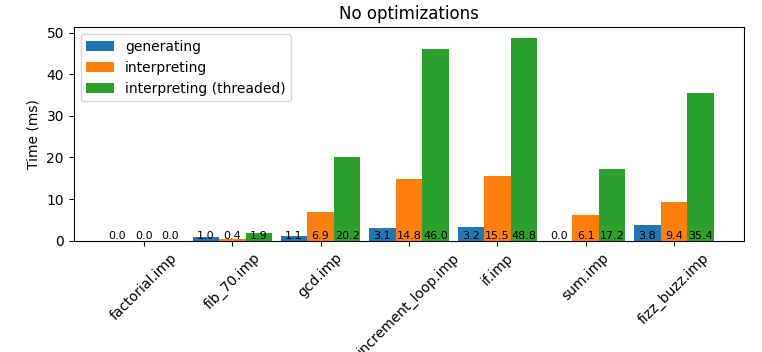
\includegraphics[width=1\textwidth]{../BenchmarkImages/No_Optimizations.png}
    \caption{Benchmark results without any optimizations enabled}
    \label{fig:no_op}
\end{figure}

\begin{figure}[h]
    \centering
    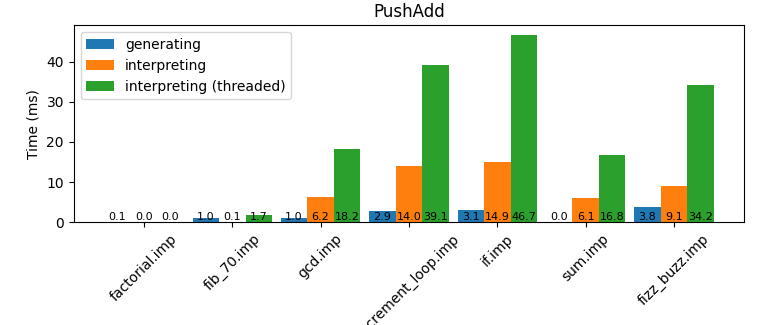
\includegraphics[width=1\textwidth]{../BenchmarkImages/PushAdd.png}
    \caption{Benchmark results with the superinstruction PushAdd enabled}
    \label{fig:push_add}
\end{figure}

\begin{figure}[h]
    \centering
    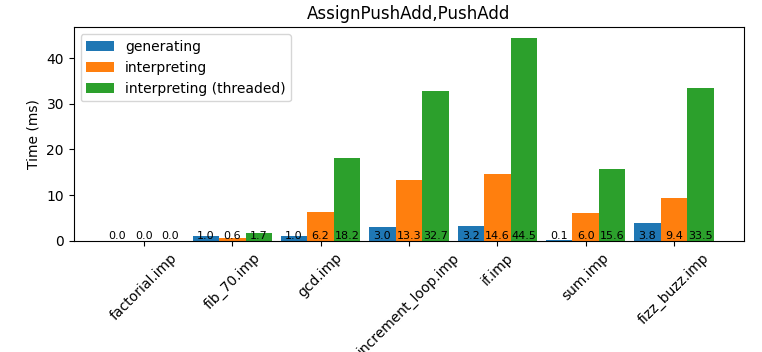
\includegraphics[width=1\textwidth]{../BenchmarkImages/AssignPushAdd_PushAdd.png}
    \caption{Benchmark results with the superinstructions PushAdd and AssignPushAdd enabled}
    \label{fig:push_add_apa}
\end{figure}

\begin{figure}[h]
    \centering
    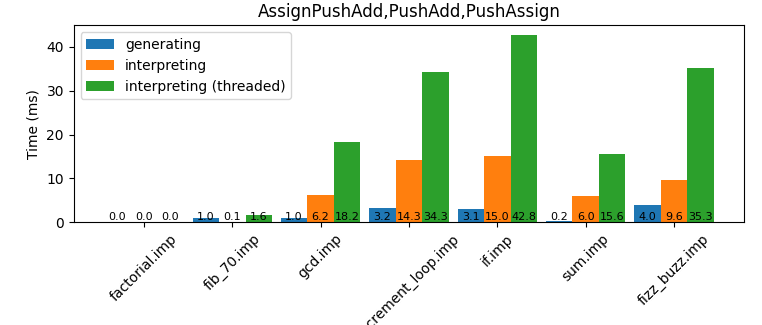
\includegraphics[width=1\textwidth]{../BenchmarkImages/AssignPushAdd_PushAdd_PushAssign.png}
    \caption{Benchmark results with the superinstructions PushAdd, AssignPushAdd and PushAssign enabled}
    \label{fig:all_op}
\end{figure}

Looking at the first diagram with no optimizations enabled we get the base
line. Now we can compare it with some of the superinstruction optimizations.

First of all, we can see that the threaded code optimization causes a slow down
of approximatly 300\% compared to the non optimized version. But why is this?
We have already explained how we have implemented the computed goto
optimization for that see Section \ref{it:goto}.

There you can see that we used a hash map to store the mapping of byte code
instruction to the function that implements it. The key is a usize. This usize
is the result of a call to the std::mem::discriminant function. It returns the
index of a given variant in an enum.

Since Rust does not by default allow an enum with fields that hold data to be
the key of a hash map we had to use this approach.

After every instruction we need to call the discriminant function to get the
index of the next byte code instruction. This overhead is most likely the main
reason for the slow down.

When we are comparing Figure \ref{fig:push_add} (PushAdd) and Figure
\ref{fig:no_op} (No optimizations) we can see that the implementation of the
superinstruction PushAdd which combines the PUSH and the ADD instruction
resulted in slight improvements in the run time.

The biggest performance benefit was gained in the increment\_loop.imp program
\ref{item:inc_loop}. The generated byte code for this program uses the
combination of pushing the value 1 to the stack and adding it to a variable in
a loop. Combining those two instructions we can gain almost a 20\% speed
improvement in the threaded code and a 6\% speed improvement in non-threaded
code.

The following shows the generated bytecode for the increment\_loop.imp program
without using any superinstructions.
\begin{verbatim}
inside the loop...

    Var("a")
    Push(1)
    Add
    Assign("a")
    Var("b")
    Push(1)
    Add
    Assign("b")
    ...
\end{verbatim}

This shows the generated bytecode using the PushAdd instruction.
\begin{verbatim}
inside the loop...

    Var("a")
    PushAdd(1)
    Assign("a")
    Var("b")
    PushAdd(1)
    Assign("b")
    ...
\end{verbatim}

As you can see we saved one instruction per incremented variable per
iteration in the loop. 

To get an even bigger performance increase on the increment\_loop.imp program
we can enable two superinstructions. As we can see in Figure
\ref{fig:push_add_apa} (PushAdd, AssignPushAdd) the run time was decreased to
only 32.7 ms in threaded code. This is an improvement in speed of nearly 30\%
in threaded code and 10\% in non-threaded code.

When we combine the previously build PushAdd superinstruction with the ASSIGN
instruction we can reduce the number of instructions even more to just two
instructions per incremented variable.

\begin{verbatim}
inside the loop...

    Var("a")
    AssignPushAdd { name: "a", value: 1 }
    Var("b")
    AssignPushAdd { name: "b", value: 1 }
    ...
\end{verbatim}

Since none of the test programs results in a generated bytecode that exceeds
100 instructions the differences at generating are minimal but in some cases
still notable.

When we compare the generation time of fizz\_buzz.imp in Figure \ref{fig:no_op}
and Figure \ref{fig:all_op} we can see that the time it took to generate the
byte code increased by 0.2ms. This increase might seem very little and
irrelevant but the generated byte code only consists of 57 instructions. If
this would be a big program resulting in thousands of instructions the time of
code generation would noticable increase as the time needed to create
superinstructions grows linear to the byte code (see Section
\ref{sec:replacing_superinstructions}).

\section{Summary}
Efficiency of an virtual machine interpreter is not just dependent on the
optimizations it implements on the generated code but also requires the virtual
machine and the interpreter to use efficient techinques. Factors like the
design of the byte code for the VM or layout of the byte code in the memory are
important factors to consider when trying to write an efficient VM interpreter.

We explored the implementation in Rust, using it's high level features. We
showed that those features, such as Rust's enums, are a convenient way to
implement a VM interpreter but might not be the most optimal approach to it.
When comparing it to how you would implement for example the byte code in C, we
can see that the technique that is not that convenient for the developer is
actually way faster and more efficent.

The same applies to the technique used to implement optimizations like the
threaded code in the interpreter.

When talking about optimizations, we showed that even simple optimizations
like superinstructions can have a measurable impact on performance. 

\section{Future Work}
\label{sec:future}
% TODO maybe run the program on other / older machines to see how it behaves there
The last section of this paper will focus on ways to improve this project
in the future.

Looking at the title of this paper and compare it to the write up we can see
that we are missing an essential part. The part of automation.

The idea behind the automation part is to give the user of this program
the opportunity to provide a configuration file which can define all 
sorts of information that then will be used for the generation of the
virutal machine interpreter.

Some of the information can be custom superinstructions for example. The idea
is to let the user define their own superinstructions and write them down in a
syntax we can understand to automatically implement them during generation.

Other ways to improve this project in the future is to think about a different
way to model the byte code inside of the Rust code as our chosen approach was
not the most efficient. 

To further improve the efficiency we can implement more optimization techniques
in the future. To name a few optimizations that should be pretty easy to
implement at this point are for example `dead code elimination` as described in
Section \ref{item:dead_code_elimination}.

Another thing that can be done in the future is to add more superinstructions.
For that it would be useful to create more benchmark examples and see what
instructions are used frequently to create superinstructions out of them.

An interesting extension to the integration of superinstructions was mentioned
in the paper 'Optimizing an ANSI C Interpreter with Superoperators'
~\cite{superoperators} where they have used a heuristic method to infer good
sets of superinstructions. This approach automates the process of finding good
superinstructions to use.

Another way to further develop this project is to change the architecture of the
virutal machine and use a register based machine. Doing this would also result
in a change of the bytecode reprentation and optimally make the VM interpreter
more efficient.

\clearpage
\bibliographystyle{plain}
\bibliography{dissertation}
\end{document}


%questions
%what to do in the video ?
%screenrecording -> run it
%what about the logbook
%images not in right position
%font correct format
%byte code or bytecode



